\documentclass[10pt,english]{article}
\usepackage[T1]{fontenc}
\usepackage[latin9]{inputenc}
\usepackage{geometry}
\geometry{verbose,tmargin=1.5in,bmargin=1.5in,lmargin=1.5in,rmargin=1.5in}
\usepackage{amsthm}
\usepackage{amsmath}
\usepackage{amssymb}
\usepackage{tikz}

\makeatletter
\usepackage{enumitem}
\newlength{\lyxlabelwidth}

\usepackage[T1]{fontenc}
\usepackage{ae,aecompl}

%\usepackage{txfonts}

\usepackage{microtype}

\usepackage{calc}
\usepackage{enumitem}
\setenumerate{leftmargin=!,labelindent=0pt,itemindent=0em,labelwidth=\widthof{\ref{last-item}}}

\makeatother

\usepackage{babel}
\begin{document}
\noindent \begin{center}
\textbf{\large{}MATH 239 - Assignment 6}\\
\textbf{\large{}Chris Ji 20725415}
\par\end{center}{\large \par}
\medskip{}

\begin{enumerate}
\item \begin{enumerate}
    \item If $P_n$ is a path graph $(V,p_n)$, where $p_n=(\{0,\ldots,n\},\{\{i-1,i|i=1,\ldots,n\})$. There are two automorphisms on $P_n$, the identity function, $f(v)=v$, and the identity function flipped, where for every $v_i\in E(P_n)$, $i\in[0,n]$, $f(v_i)=v_{n-i}$.
    
    \item You can draw each $C_n$ as a regular polygon with $n$ sides. Then from this, we can see there are $2n$ automorphisms, by rotating left or right $n$ times, and then reflecting upon each of the $n$ axes of symmetry. 
    
    \item For a complete bipartite graph $K_{n,n}$, with partitions $(A,B)$ such that every edge in $\{\{u,v\}|u\in A,v\in B\}$, there are $2(n!)^2$ automorphisms. This is because there are $n!$ ways to arrange the vertices in $A$, and $n!$ ways to arrange the vertices in $B$, and since $|A|=|B|$, then you can define $(n!)^2$ automorphisms keeping the vertices in $A$ in $A$, and then $(n!)^2$ automorphism swapping the vertices in $A$ to $B$. 
\end{enumerate}

\pagebreak
\item Partition our graph into two sets, $A$ and $B$ such that $|A|=a$, $|B|=n-a$. Then, at most, each of the vertices in $A$ are connected to $n-a$ vertices, and each of our vertices in $B$ are connected to $a$ vertices. Then by handshake lemma, the number of edges are $\frac{\sum_{a\in A}(n-a)+\sum_{b\in B}a}{2}=\frac{a(n-a)+(n-a)a}{2}=a(n-a)$. Clearly we can optimize this by taking \begin{align*}\frac{d}{da}a(n-a)&=0\\\Rightarrow n-2a&=0\\\Rightarrow a&=\frac{n}{2}\end{align*} So setting $a=\frac{n}{2}$, will give us a bipartite graph with the most edges: $\frac{n}{2}(n-\frac{n}{2})=\left(\frac{n}{2}\right)^2$, so a bipartite graph with $n$ vertices has at most $\left(\frac{n}{2}\right)^2$ edges. 

%Clearly the complete bipartite graph $k_{a,b}$, with $a,b$ being as close as possible to $\frac{n}{2}$ (if $n$ is even, they are both $\frac{n}{2}$, and if $n$ is odd, one is $\frac{n}{2} -\frac{1}{2}$, the other is $\frac{n}{2}+\frac{1}{2}$), is the bipartite graph with the most edges. The amount of edges in this is $ab$ by definition, but since $a=b=n/2$, there are $\left(\frac{n}{2}\right)^2$ edges if $n$ is even, and $\left(\frac{n}{2}-\frac{1}{2}\right)\left(\frac{n}{2}+\frac{1}{2}\right)=\left(\frac{n}{2}\right)^2-\frac{1}{4}$ if $n$ is odd. Therefore, all bipartite graphs with $n$ vertices have at most $\left(\frac{n}{2}\right)^2$ edges. 

\pagebreak
\item
\begin{enumerate}
    \item \leavevmode\vadjust{\vspace{-\baselineskip}}\newline
    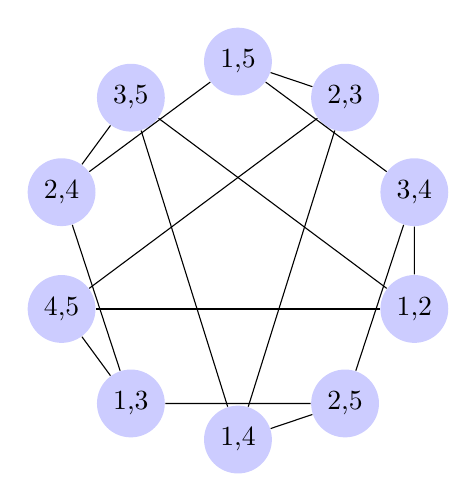
\begin{tikzpicture}
  [scale=.8,auto=left,every node/.style={circle,fill=blue!20},baseline]
  \node (n1) at (2.8,-0.927)   {1,2};
  \node (n2) at (-1.7,-2.427)   {1,3};
  \node (n3) at (0,-3)    {1,4};
  \node (n4) at (0,3)    {1,5};
  \node (n5) at (1.7,2.427)         {2,3};
  \node (n6) at (-2.8,0.927)  {2,4};
  \node (n7) at (1.7,-2.427)  {2,5};
  \node (n8) at (2.8,0.927)   {3,4};
  \node (n9) at (-1.7,2.427)   {3,5};
  \node (n10) at (-2.8,-0.927)         {4,5};

  \foreach \from/\to in {n1/n8,n1/n9,n1/n10,n2/n6,n2/n7,n2/n10,n3/n5,n3/n7,n3/n9,n4/n5,n4/n6,n4/n8,n5/n10,n6/n9,n7/n8}
    \draw (\from) -- (\to);
\end{tikzpicture}

\begin{tikzpicture}
  [scale=.8,auto=left,every node/.style={circle,fill=blue!20},baseline]
  \node (n1) at (5,0) {1,2};
  \node (n2) at (4.5,2)  {1,3};
  \node (n3) at (3.3,3.7)  {1,4};
  \node (n4) at (1.5,4.7) {1,5};
  \node (n5) at (-0.5,5)  {2,3};
  \node (n6) at (-2.5,4.3)  {2,4};
  \node (n7) at (-4,2.9)  {2,5};
  \node (n8) at (-4.9,1)  {3,4};
  \node (n9) at (-4.9,-1)  {3,5};
  \node (n10) at (-4.1,-2.9)  {4,5};
  \node (n11) at (-2.5,-4.3)  {1,6};
  \node (n12) at (-0.5,-5)  {2,6};
  \node (n13) at (1.5,-4.7)  {3,6};
  \node (n14) at (3.3,-3.7)  {4,6};
  \node (n15) at (4.5,-2)  {5,6};

  \foreach \from/\to in {n1/n8,n1/n9,n1/n10,n2/n6,n2/n7,n2/n10,n3/n5,n3/n7,n3/n9,n4/n5,n4/n6,n4/n8,n5/n10,n6/n9,n7/n8,n1/n13,n1/n14,n1/n15,n2/n12,n2/n14,n2/n15,n3/n12,n3/n13,n3/n15,n4/n12,n4/n13,n4/n14,n5/n11,n5/n14,n5/n15,n6/n11,n6/n14,n6/n15,n7/n11,n7/n14,n8/n11,n8/n12,n8/n15,n9/n11,n9/n12,n9/n14,n10/n11,n10/n12,n10/n13,n7/n13,n6/n13,}
    \draw (\from) -- (\to);
\end{tikzpicture} \\ PS: Please let the solutions have a symmetric graph for $S_{6,2}$, even the one for $S_{5,2}$ warms my heart for how pretty it is
    \item The degrees of the vertices is ${n-k\choose k}$. This is because there are $n-k$ numbers other than the ones in the vertex, and there are $k$ numbers in the vertex. 
    \item There are $\frac{{n\choose k}{n-k\choose k}}{2}$ edges. There are ${n\choose k}$ vertices, each vertex has ${n-k\choose k}$ edges, and since each edge connects 2 vertices, we divide by 2. 
\end{enumerate}

\pagebreak
\item $\Phi:V(G)\rightarrow V(H_2)$ can be defined as: $\Phi(1)=W,\Phi(2)=E,\Phi(3)=L,\Phi(4)=C,\Phi(5)=O,\Phi(6)=M,\Phi(7)=I,\Phi(8)=N,\Phi(9)=G$. $H_1$ is not isomorphic to $G$, as since $G$ and $9$ are the only two vertices with 2 neighbours, for an isomorphism $\Phi:H_1\rightarrow G$, $\Phi(G)$ must be equal to $9$. But then $N,C$ should be isomorphic to $4,8$, in any order, but $5$, a common neighbour of $4,8$ in $G$ has a neighbourhood of size 3, but $O$, a common neighbour of $N,C$ in $H_1$, has a neighbourhood of size 4. 

\pagebreak
\item Obviously, if $(v_o,\ldots,v_k)$ is a path, then $\text{deg}_G(v_0)\geq1$. If $\text{deg}_G(v_0)=1$, then the first condition is true, and if $\text{deg}_G(v_0)>1$, then  $v_0$ has neighbours. If all of $v_0$'s neighbours are in the path, then $G$ has to contain a cycle, as the neighbours of $v_0$ have to be connected, and since they are connected outside $v_0$, and through $v_0$ (since they are neighbours), that is a cycle (fulfilling condition three). Otherwise, $v_0$ has a neighbour not on the path, fulfilling the second condition. 
\end{enumerate}

\end{document}
